Die folgenden Experimente wurden zum Überprüfen der Leistungsfähigkeit des Algorithmus entwickelt. Im Kern stehen sich immer zwei gleich große Gruppen von Agenten gegenüber, deren Ziel es ist die Startpositionen der Agenten der anderen Gruppen zu erreichen. Die Anzahl der Agenten variiert zwischen den Experimenten und der freie Raum wird tendenziell immer kleiner. Für jedes Experiment ist es das Ziel, dass in allen 30 Wiederholung eine Lösung gefunden wird, also alle Agenten ihr Ziel erreichen.

Der Aufbau der Experimente und das zu erwartende Verhalten der Agenten werden vorgestellt. Im Kapitel \ref{chap:ergebnisse} folgen dann die Messwerte aus \cite{book:regele} und die eigenen.

\subsection{Sechs gegen sechs: Lockere Vorbeifahrt}
\label{chap:6x6_locker}
Das erste Experiment dieser Reihe bietet vergleichsweise viel Platz. Es ist vor allem für den späteren Vergleich interessant.

\textbf{Aufbau des Experiments}
\begin{figure}[H]
    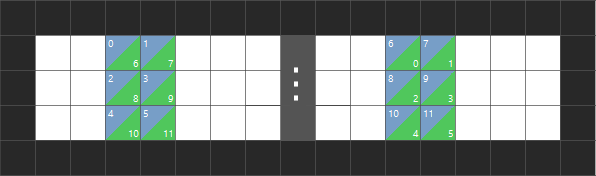
\includegraphics[width=\textwidth]{images/6vs6_spacy.png}
    \centering
    \caption{Aufbau für die lockere Vorbeifahrt zweier Gruppen, bestehend aus jeweils sechs Agenten}
    \label{fig:6x6Locker}
\end{figure}
 Die Abbildung \ref{fig:6x6Locker} zeigt eine Karte die drei mal 30 Felder misst. Es stehen sich zwei Gruppen, bestehend aus jeweils sechs Agenten, gegenüber. Zum rechten beziehungsweise linken Rand sind für die Gruppen noch ein paar freie Felder vorhanden. Damit soll es den Agenten möglich sein, Ausweichbewegungen nach hinten hin ausführen zu können.
\subsection{Sechs gegen sechs: Enge Vorbeifahrt}
\label{chap:6x6_eng}
In diesem Experiment ist der Platz für Bewegungen sehr beschränkt. Zwölf Felder sind von Agenten belegt und lediglich neun sind frei. 

\textbf{Aufbau des Experiments}
\begin{figure}[H]
    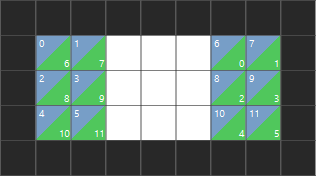
\includegraphics[height=40mm]{images/6vs6_tight.png}
    \centering
    \caption{Aufbau für die enge Vorbeifahrt zweier Gruppen, bestehend aus jeweils sechs Agenten}
    \label{fig:6x6Eng}
\end{figure}
Die Karte für dieses Experiment ist sieben mal drei Felder groß. Es stehen sich zwei Gruppen aus jeweils sechs Agenten gegenüber. Wie in Abbildung \ref{fig:6x6Eng} zu erkennen, befindet sich zwischen den beiden Gruppen ein Block aus drei mal drei freien Feldern.
\subsection{Drei gegen drei: Enge Vorbeifahrt}
\label{chap:3x3_eng}
Dieses Experiment dient als Vergleich zum Vorangegangenen. Die Auswirkung die die Anzahl der Roboter hat, soll hiermit untersucht werden. 

\textbf{Aufbau des Experiments}
\begin{figure}[H]
    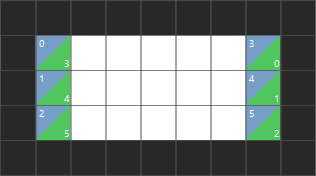
\includegraphics[height=40mm]{images/3vs3.png}
    \centering
    \caption{Aufbau für die enge Vorbeifahrt zweier Gruppen, bestehend aus jeweils drei Agenten}
    \label{fig:3x3}
\end{figure}
Die Karte für dieses Experiment ist sieben mal drei Felder groß. Es stehen sich zwei Gruppen aus jeweils drei Agenten gegenüber. Wie in Abbildung \ref{fig:3x3} zu erkennen, befindet sich zwischen den beiden Gruppen ein Block aus fünf mal drei freien Feldern.
\subsection{Vier gegen vier: Enge Vorbeifahrt}
\label{chap:4x4_eng}
Dieses Experiment schränkt den Platz der Agenten weiter ein. Die Zahl der belegten Felder ist hier größer als die Anzahl der freien Felder. Besonders für dieses Experiment ist, dass ein Graph vorliegt der die Prioritätswerte der Agenten über die Zeit zeigt (siehe Abbildung \ref{tab:resultsCoDy} und \ref{tab:myResults}). 

\textbf{Aufbau des Experiments}
\begin{figure}[H]
    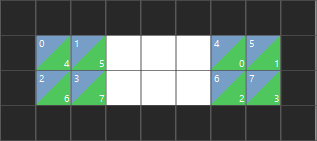
\includegraphics[height=32mm]{images/4vs4_tight.png}
    \centering
    \caption{Aufbau für die enge Vorbeifahrt zweier Gruppen, bestehend aus jeweils vier Agenten}
    \label{fig:4x4}
\end{figure}
Die Karte für dieses Experiment misst sieben mal zwei Felder. Acht Agenten teilen sich in zwei gleich große Gruppen und stehen sich gegenüber.
\subsection{Messergebnisse}
\label{chap:ergebnisse}
\begin{table}[H]
    \centering
    \begin{tabular}{c|c|c|c|c|c|c}
       \textbf{Experiment} & \textbf{Gelöst} & \textbf{Prioritäts-Überlauf}
        & \(\textbf{s\textsubscript{opt}}\) & \(\textbf{s\textsubscript{CoDy}}\)
        & \(\textbf{t\textsubscript{opt}}\) & \(\textbf{t\textsubscript{CoDy}}\)\\ \hline
       \textbf{6-vs-6-locker} & 30 von 30 & 0 von 30
       & 19.5 & 20.97 & 22 & 24.33 \\ \hline
       \textbf{6-vs-6-eng} & 26 von 30 & 1 von 30
       & 5.45 & 11.5 & 10.35 & 21.89 \\ \hline
       \textbf{3-vs-3-eng} & 30 von 30 & 3 von 30
       & 5.5 & 6.35 & 6.33 & 7.68 \\ \hline
       \textbf{4-vs-4-eng} & 27 von 30 & 4 von 30
       & 5 & 10.85 & 10.5 & 24.96
    \end{tabular}
    \caption{Messwerte der Experimente aus \cite{book:regele}}
    \label{tab:resultsCoDy}
\end{table}

\begin{table}[H]
    \centering
    \begin{tabular}{c|c|c|c|c}
       \textbf{Experiment} & \textbf{Gelöst} & \textbf{Prioritäts-Überlauf}
        & [\textbf{\(\bar{s}\textsubscript{u}\)}, \textbf{\(\bar{s}\textsubscript{o}\)}]
        & [\textbf{\(\bar{t}\textsubscript{u}\)}, \textbf{\(\bar{t}\textsubscript{o}\)}]\\ \hline
       \textbf{6-vs-6-locker} & 30 von 30 & 0 von 30 & [20.01, 22.33] & [23.92, 26.4]\\ \hline
       \textbf{6-vs-6-eng} & 18 von 30 & 18 von 18 & [8.78, 9.81] & [19.52, 23.09]\\ \hline
       \textbf{3-vs-3-eng} & 27 von 30 & 0 von 27 & [7.3, 7.58] & [9.53, 9.97]\\ \hline
       \textbf{4-vs-4-eng} & 20 von 30 & 20 von 20 & [13.72, 25.2] & [23.04, 41.04]
    \end{tabular}
    \caption{Messwerte der selbst durchgeführten Experimente}
    \label{tab:myResults}
\end{table}

Die eigenen Messwerte weichen teils stark von den vorgegeben Messwerten ab. Lediglich das Experiment "'\ref{chap:6x6_locker} Sechs gegen sechs: Lockere Vorbeifahrt"' trifft die Erwartungen.

Für die eigenen Messungen ist anzumerken, dass für den Prioritätsüberlauf nicht immer "'von 30"' angegeben ist. Das hat damit zu tun, dass die Simulationsumgebung nur Daten erzeugt, wenn ein Experiment erfolgreich war.

\begin{figure}[H]
    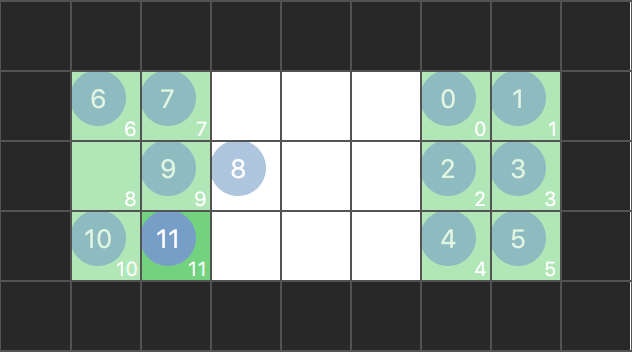
\includegraphics[height=40mm]{images/6vs6_tight_full_block.png}
    \centering
    \caption{Beispielhafte Totalblockade für das Experiment "'\ref{chap:6x6_eng} Sechs gegen sechs: Enge Vorbeifahrt"'}
    \label{fig:6x6EngFullBlock}
\end{figure}
Für das Experiment "'\ref{chap:6x6_eng} Sechs gegen sechs: Enge Vorbeifahrt"' ist der zurückgelegte Strecke etwas besser als erwartet. Der Zeitbedarf trifft die Erwartung. Auffällig ist jedoch, dass nur 18 statt 26 Wiederholungen erfolgreich sind und es in allen, statt nur bei einer Wiederholung, zu Prioritätsüberläufen kam. Bei den zwölf ungelösten Wiederholungen ist eine Variation der in Abbildung \ref{fig:6x6EngFullBlock} gezeigten Situation eingetreten. 

Die Werte für "'\ref{chap:3x3_eng} Drei gegen drei: Enge Vorbeifahrt"'
weichen nur leicht von den erwarteten ab. Statt 30 werden nur 27 Wiederholungen gelöst. Dafür kommt es in den gelösten Wiederholungen aber nicht zu Prioritätsüberläufen. Die drei erwarteten Wiederholungen, die einen Prioritätsüberläufen haben, entstehen aus Situationen, in denen sich die Agenten in breiter Front aufeinander zu bewegen. In den eigenen Experimenten führten genau diese Situation zu den drei ungelösten Wiederholungen.

Die gemessenen Werte weichen für das Experiment "'\ref{chap:4x4_eng} Vier gegen vier: Enge Vorbeifahrt"' am stärksten ab. Es werden nur in 20 statt 27 Wiederholungen Lösungen gefunden. In jeder Wiederholung kommt es zu Prioritätsüberläufen. Auch das war nicht erwartet. Die Konfidenzintervalle für die durchschnittlich zurückgelegte Strecke und den durchschnittlichen Zeitbedarf sind im Vergleich besonders groß. Die erwartete Strecke ist nicht mal im Intervall enthalten. Wie Abbildungen \ref{fig:4x4_prio_2} deutlich zeigt, wird der erwartete Prioritätsverlauf verfehlt. Statt das die Priorität der Agenten über die Zeit stetig ansteigt und teilweise wieder zurückgeht, pendeln bei den eigenen Experimenten die Prioritätswerte zwischen minimalen und maximalen Werten hin und her.

\begin{figure}[H]
    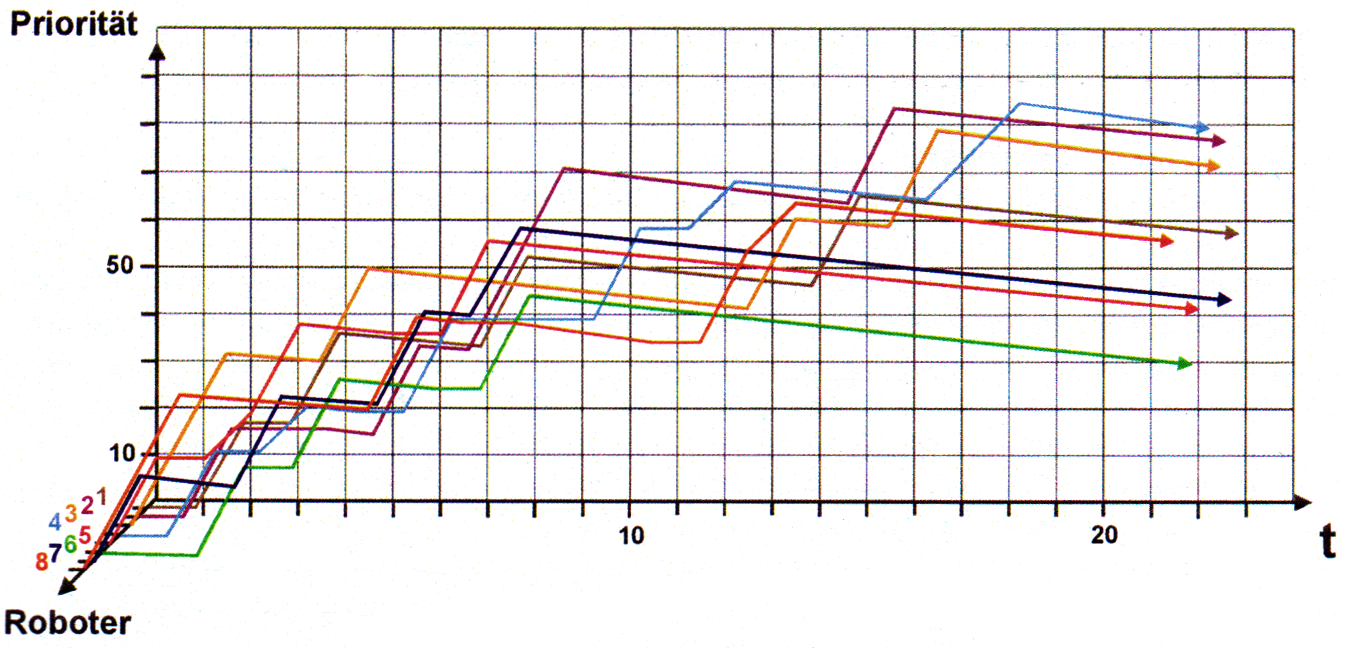
\includegraphics[width=\textwidth]{images/4vs4_tight_prio_ref.png}
    \centering
    \caption{Prioritätsverlauf aller Agenten für das Experiment "'\ref{chap:4x4_eng} Vier gegen vier: Enge Vorbeifahrt"' aus \cite{book:regele}}
    \label{fig:4x4_prio_1}
\end{figure}

\begin{figure}[H]
    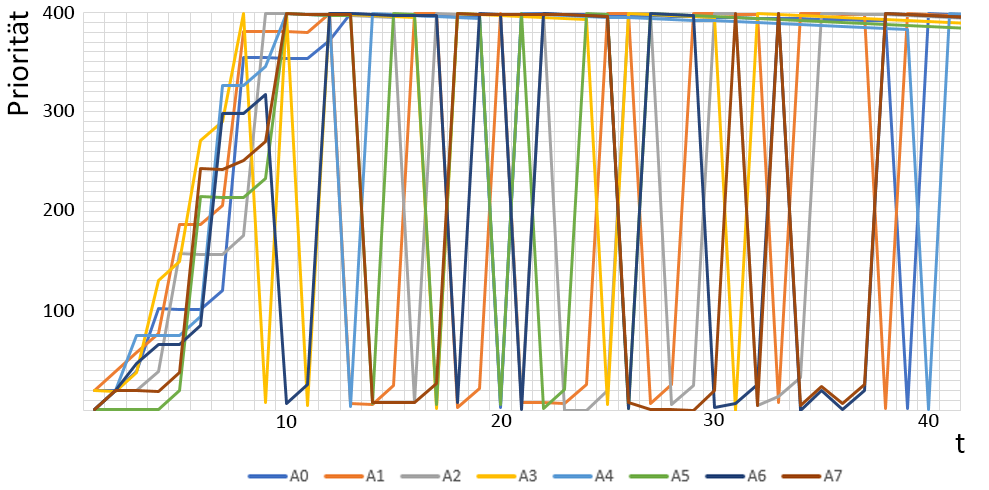
\includegraphics[width=\textwidth]{images/4vs4_tight_prio.png}
    \centering
    \caption{Prioritätsverlauf aller Agenten für das Experiment "'\ref{chap:4x4_eng} Vier gegen vier: Enge Vorbeifahrt"' der selbst durchgeführten Experimente}
    \label{fig:4x4_prio_2}
\end{figure}